%%%%%%%%%%%%%%%%%%%%%%%%%%%%%%%%%%%%%%%%%%%%%%%%%%%%%%%%%%%%%%%%%%%%%%%%%%%%%%%%%%%%%%%%%%%%%%%%%%%%%%%%%%%%%%%%%%%%%%%%%%%%%%%%%%%%%%%%%%%%%%%%%%%%%%%%%%%
% This is just an example/guide for you to refer to when producing your supplementary material for your Frontiers article.                                 %
%%%%%%%%%%%%%%%%%%%%%%%%%%%%%%%%%%%%%%%%%%%%%%%%%%%%%%%%%%%%%%%%%%%%%%%%%%%%%%%%%%%%%%%%%%%%%%%%%%%%%%%%%%%%%%%%%%%%%%%%%%%%%%%%%%%%%%%%%%%%%%%%%%%%%%%%%%%

%%% Version 2.5 Generated 2018/06/15 %%%
%%% You will need to have the following packages installed: datetime, fmtcount, etoolbox, fcprefix, which are normally inlcuded in WinEdt. %%%
%%% In http://www.ctan.org/ you can find the packages and how to install them, if necessary. %%%
%%%  NB logo1.jpg is required in the path in order to correctly compile front page header %%%

\documentclass[utf8]{frontiers_suppmat} % for all articles
\usepackage{url,hyperref,lineno,microtype}
\usepackage[onehalfspacing]{setspace}
\usepackage[outdir=./]{epstopdf}

%\usepackage{caption}
%\captionsetup[table]{font=normalsize}



% Leave a blank line between paragraphs instead of using \\

\begin{document}

\onecolumn
\firstpage{1}

\title[Supplementary Material]{{\helveticaitalic{Supplementary Material}}}
%\subtitle{Preferences for income redistribution in unequal contexts: Changes in Latin America between 2008 and 2018}

\maketitle


%\section{Appendix 1}

\begin{table}[h]
\centering
	\caption{Sample: Observations by country and year.}
	\label{appendix1}
	\renewcommand{\arraystretch}{0.8}
    \begin{tabular}{lrrrrrrr}
     \toprule
     & 2008 & 2010 & 2012 & 2014 & 2016 & 2018 & Total \\
		\midrule
		Argentina & 1028 & 1041 & 1027 & 868 & 1123 & 1260 & 6347 \\
		Bolivia & 2487 & 2408 & 2473 & 2356 & 1407 & 1440 & 12571 \\
		Brazil & 1234 & 2142 & 1369 & 1344 & 1305 & 1264 & 8658 \\
		Chile & 1288 & 1620 & 1301 & 1108 & 1410 & 1377 & 8104 \\
		Colombia & 1213 & 1322 & 1197 & 1355 & 1275 & 1302 & 7664 \\
		Costa Rica & 1252 & 1083 & 1032 & 1104 & 1258 & 1320 & 7049 \\
		Dominican Republic & 1165 & 1246 & 1244 & 1296 & 1147 & 1278 & 7376 \\
		Ecuador & 2674 & 2728 & 1329 & 1273 & 1238 & 1281 & 10523 \\
		El Salvador & 1427 & 1451 & 1193 & 1272 & 1322 & 1209 & 7874 \\
		Guatemala & 1059 & 1146 & 1088 & 1212 &  &  &  \\
		Honduras & 1233 & 1458 & 1299 & 1369 & 1187 & 1083 & 7629 \\
		Mexico & 1288 & 1336 & 1232 & 1130 & 1317 & 1331 & 7634 \\
		Nicaragua &  & 1258 & 1447 & 1359 &  &  &  \\
		Panama & 1355 & 1434 & 1314 & 1374 & 1306 & 1338 & 8121 \\
		Paraguay & 988 & 1073 & 1274 & 1082 & 1049 & 1294 & 6760 \\
		Peru & 1337 & 1343 & 1291 & 1138 & 2299 & 1320 & 8728 \\
		Uruguay & 1328 & 1370 & 1314 & 1378 & 1353 & 1437 & 8180 \\
		Total & 22356 & 25459 & 22424 & 22018 & 19996 & 19534 & 131787 \\
		\bottomrule
	\end{tabular}
\end{table}

\newpage

%\section{Appendix 2}

\begin{table}[h]
\centering
	\caption{Within and between-country distribution of dependent and independent variables.}
	\label{appendix2}
    \renewcommand{\arraystretch}{0.8}
\begin{tabular}{lrrrrrrr}
  \toprule
	 & \multicolumn{3}{c}{Support for redistribution} & \multicolumn{2}{c}{GINI} & \multicolumn{2}{c}{GDP per capita} \\
    Country & Mean & SD total & SD years & Mean & SD years & Mean & SD years \\
  \midrule
  Argentina & 5.86 & 1.55 & 0.25 & 42.42 & 1.38 & 13.47 & 0.25 \\ 
  Bolivia & 5.25 & 1.55 & 0.27 & 47.38 & 2.15 & 2.83 & 0.32 \\ 
  Brazil & 5.76 & 1.62 & 0.25 & 53.32 & 0.60 & 8.71 & 0.33 \\ 
  Chile & 5.99 & 1.35 & 0.20 & 45.77 & 1.07 & 12.88 & 0.89 \\ 
  Colombia & 5.76 & 1.53 & 0.25 & 52.57 & 1.99 & 5.72 & 0.50 \\ 
  Costa Rica & 5.84 & 1.62 & 0.30 & 48.50 & 0.18 & 11.18 & 0.88 \\ 
  Dominican Republic & 5.93 & 1.56 & 0.24 & 46.20 & 1.22 & 6.50 & 0.90 \\ 
  Ecuador & 5.46 & 1.65 & 0.29 & 46.57 & 2.00 & 5.77 & 0.35 \\ 
  El Salvador & 5.68 & 1.58 & 0.27 & 41.97 & 2.78 & 3.59 & 0.21 \\ 
  Guatemala & 5.40 & 1.69 & 0.24 & 54.36 & 0.64 & 3.71 & 0.12 \\ 
  Honduras & 5.21 & 1.85 & 0.17 & 51.85 & 2.28 & 2.27 & 0.12 \\ 
  Mexico & 5.65 & 1.62 & 0.23 & 47.85 & 1.35 & 9.41 & 0.35 \\ 
  Nicaragua & 5.83 & 1.65 & 0.30 & 48.22 & 1.04 & 1.84 & 0.12 \\ 
  Panama & 5.51 & 1.73 & 0.47 & 51.13 & 0.95 & 12.38 & 1.85 \\ 
  Paraguay & 5.71 & 1.70 & 0.57 & 49.40 & 1.43 & 5.13 & 0.50 \\ 
  Peru & 5.42 & 1.56 & 0.27 & 44.57 & 1.54 & 5.80 & 0.63 \\ 
  Uruguay & 5.82 & 1.60 & 0.34 & 41.47 & 2.37 & 14.58 & 1.45 \\ 
  Total & 5.63 & 1.63 &  & 47.71 & 4.17 & 7.65 & 4.12 \\ 
		\bottomrule
	\end{tabular}
\end{table}

\newpage

%\section{Appendix 3}

\begin{figure}[h]
	\centering
		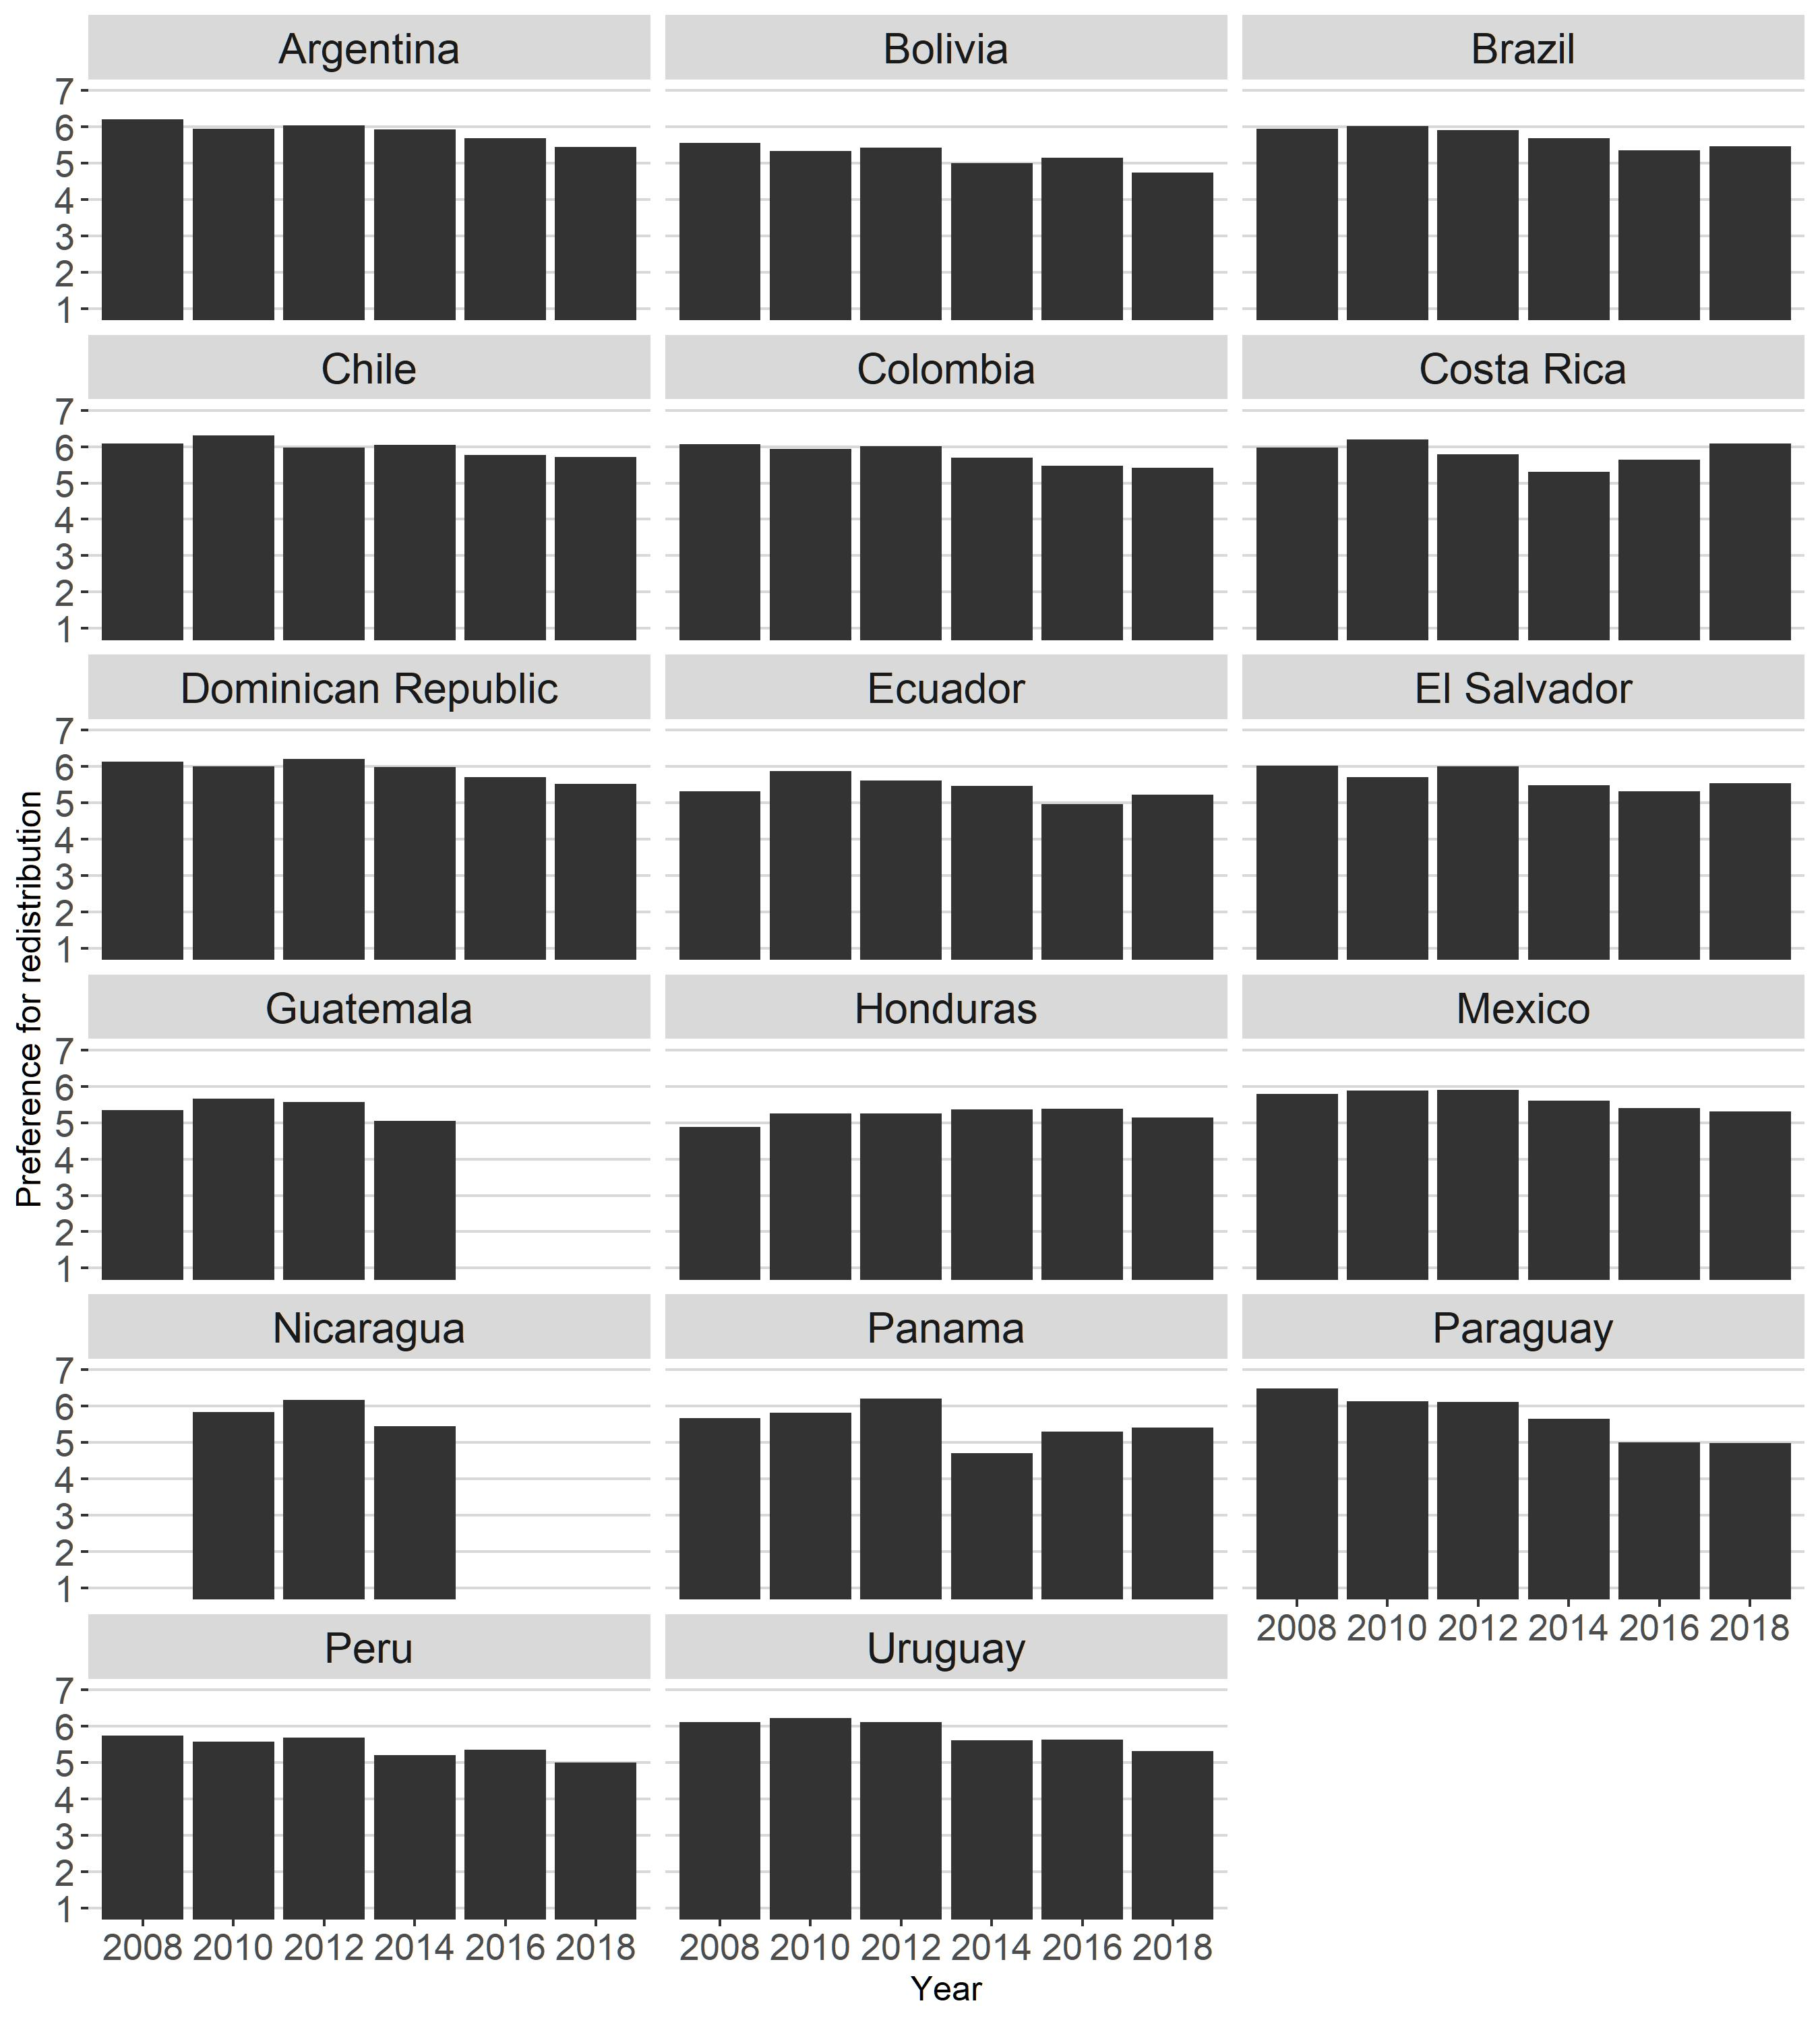
\includegraphics[,width=0.95\textwidth]{./Output/Graphs/Appendix3.jpg}
		\caption{Average support for redistribution, by country and year.}
		\label{appendix3}
\end{figure}

\newpage

%\section{Appendix 4}

\begin{table}[h]
\centering
\caption{Hybrid multilevel regression models of individual support for redistribution. Continuous, categorical and quadratic income measures.}
\label{appendix4}
\renewcommand{\arraystretch}{0.8}
\begin{tabular}{l D{.}{.}{7.5} D{.}{.}{7.5} D{.}{.}{7.5}}
\toprule
 & \multicolumn{1}{c}{Model 1} & \multicolumn{1}{c}{Model 2} & \multicolumn{1}{c}{Model 3}\\
\midrule
Income                       & 0.00^{*}    &             & 0.03^{***}  \\
                             & (0.00)      &             & (0.01)      \\
Income^2                     &             &             & -0.00^{***} \\
                             &             &             & (0.00)      \\
Income\_Decile2              &             & 0.04^{**}   &             \\
                             &             & (0.02)      &             \\
Income\_Decile3              &             & 0.05^{***}  &             \\
                             &             & (0.02)      &             \\
Income\_Decile4              &             & 0.06^{***}  &             \\
                             &             & (0.02)      &             \\
Income\_Decile5              &             & 0.08^{***}  &             \\
                             &             & (0.02)      &             \\
Income\_Decile6              &             & 0.05^{**}   &             \\
                             &             & (0.02)      &             \\
Income\_Decile7              &             & 0.06^{***}  &             \\
                             &             & (0.02)      &             \\
Income\_Decile8              &             & 0.06^{***}  &             \\
                             &             & (0.02)      &             \\
Income\_Decile9              &             & 0.10^{***}  &             \\
                             &             & (0.02)      &             \\
Income\_Decile10             &             & 0.02        &             \\
                             &             & (0.02)      &             \\
\hline
Constant                     & 5.40^{***}  & 5.36^{***}  & 5.35^{***}  \\
                             & (0.08)      & (0.08)      & (0.09)      \\
\hline
Individual-level controls    &     Yes     &     Yes     &     Yes     \\
Year fixed effects           &     Yes     &     Yes     &     Yes     \\
\hline
AIC                          & 501403.54   &  501438.84  & 501408.03   \\
BIC                          & 501618.89   &  501732.51  & 501633.17   \\
Log Likelihood               & -250679.77  & -250689.42  & -250681.01  \\
N Level 1                    & 131787      & 131787      & 131787      \\
N Level 2                    & 97          & 97          & 97          \\
N Level 3                    & 17          & 17          & 17          \\
Var: Level 2 (Int)           & 0.05        & 0.05        & 0.05        \\
Var: Level 3 (Int)           & 0.05        & 0.05        & 0.05        \\
Var: Residual                & 2.49        & 2.49        & 2.49        \\
\bottomrule
\multicolumn{4}{l}{\scriptsize{$^{***}p<0.01$, $^{**}p<0.05$, $^*p<0.1$}}
\end{tabular}
\end{table}


\end{document}
